\documentclass[11pt]{article}

\usepackage[margin=2.5cm]{geometry}
\usepackage{amsmath,amssymb,amsthm,mathtools}
\usepackage{enumitem}
\usepackage{booktabs}
\usepackage{graphicx}
\usepackage{hyperref}

\newtheorem{theorem}{Theorem}[section]
\newtheorem{proposition}[theorem]{Proposition}
\newtheorem{lemma}[theorem]{Lemma}
\newtheorem{corollary}[theorem]{Corollary}
\newtheorem{conjecture}[theorem]{Conjecture}
\theoremstyle{definition}
\newtheorem{definition}[theorem]{Definition}
\newtheorem{example}[theorem]{Example}
\newtheorem{remark}[theorem]{Remark}

\newcommand{\One}{\textsc{One}}
\newcommand{\All}{\textsc{All}}
\newcommand{\N}{\mathbb{N}}
\newcommand{\R}{\mathbb{R}}
\newcommand{\Bin}{\mathrm{Bin}}
\newcommand{\Prob}{\mathbb{P}}
\DeclareMathOperator{\Hent}{H}

\title{Convergence and magic numbers:\\
       the optimal value of the all-heads coin game below the fair coin}
\author{Peter Pfaffelhuber}
\date{\today}

\begin{document}
\maketitle

\begin{abstract}
  In the all-heads coin game a player tosses a pool of $n$ coins, each
  landing heads with probability~$p$, must set aside at least one head
  each round, and loses on an all-tails round; $w_{n,p}$ denotes the
  optimal winning probability.  We prove that $n\mapsto w_{n,p}$
  converges for \emph{every} $p\in(0,1)$.  The proof is a three-line
  consequence of an exact identity for the increment
  $w_{n,p}-w_{n-1,p}$, which shows that every decrease is bounded by
  $q^n$, $q=1-p$.  For $p<\tfrac12$ the sequence is nevertheless not
  eventually monotone: it decreases infinitely often, but the total
  decrease is summable.  This is in sharp contrast to the greedy
  strategy, whose value oscillates log-periodically without converging;
  the optimal player cancels that oscillation exactly.  The optimal
  policy has a transparent structure: with $j$ tails the player keeps
  the smallest \emph{magic number} $\ge j$ --- a suffix-maximum record
  of $w_{n,p}$ --- and plays \One{} if there is none; we prove that
  there are infinitely many magic numbers, with $M_{k+1}\le C(p)M_k$.  We derive the exact
  criterion for the birth of a magic number, a two-phase description
  of the dynamics between births, and a heuristic law
  $M_{k+1}/M_k\to r(p)$ for the growth of magic numbers, confirmed
  numerically to within a few percent across $0.15\le p\le0.47$.
\end{abstract}

%% =====================================================================
\section{Introduction}\label{sec:intro}
%% =====================================================================

\subsection{The game}

Fix $p\in(0,1)$ and write $q:=1-p$.  A player holds $n$ coins, each of
which lands heads independently with probability~$p$.  In each round
all remaining coins are tossed; the player must set aside at least one
coin showing heads, and loses if no coin shows heads.  The game is won
once every coin has been set aside.  Writing $w_{n,p}$ for the optimal
winning probability, the dynamic-programming principle gives the
Bellman equation
\begin{equation}\label{eq:bellman}
  w_{n,p}=p^{n}+\sum_{j=1}^{n-1}\binom{n}{j}p^{\,n-j}q^{\,j}
          \max_{j\le m\le n-1}w_{m,p},\qquad w_{0,p}:=1 ,
\end{equation}
obtained by conditioning on the number $j$ of tails in the first
round: the player then keeps some number $m\in\{j,\dots,n-1\}$ of
coins (setting aside $n-m$ of the $n-j$ heads) and continues
optimally from state~$m$.  Two strategies are natural: \One{} sets
aside a single head each round (value $a_{n,p}$), and the greedy
strategy \All{} sets aside \emph{every} head (value $b_{n,p}$):
\begin{equation}\label{eq:abrec}
  a_{n,p}=p^{n}+(1-p^{n}-q^{n})\,a_{n-1,p},
  \qquad
  b_{n,p}=p^{n}+\sum_{j=1}^{n-1}\binom{n}{j}p^{\,n-j}q^{\,j}\,b_{j,p},
  \qquad a_{0,p}=b_{0,p}:=1 .
\end{equation}
The companion paper~\cite{Paper1} determines $w_{n,p}$ exactly at
$p=\tfrac12$ (it equals $\tfrac12$), shows that \One{} is optimal and
$w_{n,p}$ strictly increasing for $p>\tfrac12$, and gives a
first-order perturbation expansion for $p<\tfrac12$ near $\tfrac12$;
all of those results are machine-checked in Lean~4.  The large-$n$
asymptotics of the greedy strategy are the subject of~\cite{Paper2}:
for $p<\tfrac12$, $b_{n,p}=\Phi_p(\log n)(1+O(1/n))$ with $\Phi_p$
continuous and $\log(1/q)$-periodic, and $\Phi_p$ is non-constant at
first order in $\tfrac12-p$ --- the greedy value oscillates and does
not converge.  A coin-flipping game with a related but distinct
scoring rule is studied by van~Doorn~\cite{vanDoorn}.

The present paper concerns the large-$n$ behaviour of the
\emph{optimal} value for $p<\tfrac12$.  The natural guess, given the
greedy asymptotics, is that $w_{n,p}$ oscillates as well.  It does
not.

\subsection{Main results}\label{sec:main}

\begin{theorem}[convergence]\label{thm:conv}
  For every $p\in(0,1)$ the limit $W(p):=\lim_{n\to\infty}w_{n,p}$
  exists.  Moreover, for every $n\ge1$,
  \begin{equation}\label{eq:dipbound}
    w_{n-1,p}-w_{n,p}\;\le\;q^{\,n}\,w_{n-1,p}\;\le\;q^{\,n},
  \end{equation}
  and $\sum_{n\ge1}|w_{n,p}-w_{n-1,p}|\le 1+q/p$.
\end{theorem}

\begin{theorem}[infinitely many decreases]\label{thm:dips}
  For every $p\in(0,\tfrac12)$ the sequence $n\mapsto w_{n,p}$ is not
  eventually non-decreasing: $w_{n,p}<w_{n-1,p}$ for infinitely
  many~$n$.
\end{theorem}

A third unconditional result concerns the \emph{records} of the
sequence, the states $m$ with $w_m>w_k$ for all $k>m$, which we call
magic numbers because they are exactly the states an optimal player
reduces the pool to (Proposition~\ref{prop:policy}).

\begin{theorem}[infinitely many magic numbers]\label{thm:magic-inf-intro}
  For every $p\in(0,\tfrac12)$ there are infinitely many magic numbers
  $M_1<M_2<\cdots$, and $M_{k+1}\le C(p)M_k$ for large $k$, with
  $C(p)$ the root $r>1$ of $(r-1)\log(q/p)=rH(1/r)$
  (Theorem~\ref{thm:magic-inf}).
\end{theorem}

Theorems~\ref{thm:conv} and~\ref{thm:dips} together describe a
sequence that converges but is not eventually monotone, with
decreases that are individually exponentially small and collectively
summable.  Both rest on a single exact identity for the increment
(Lemma~\ref{lem:increment}), whose two error terms have definite
signs.  The proof of Theorem~\ref{thm:conv} is three lines long once
the identity is written down, and is well suited to formal
verification.

The contrast with the greedy strategy is striking and, at first
sight, paradoxical: $w_{n,p}\ge b_{n,p}$, $b_{n,p}$ oscillates with an
amplitude of order $10^{-6}$ at $p=0.45$ (and larger for smaller~$p$),
yet $w_{n,p}$ converges --- the optimal player cancels the greedy
oscillation exactly.  Section~\ref{sec:magic} explains how.  The
Bellman maximum in~\eqref{eq:bellman} is attained at a \emph{record}
of the value sequence, and the optimal policy is entirely described by
the set of records, which we call \emph{magic numbers}: with $j$ tails
the player reduces the pool to the smallest magic number $\ge j$
(Proposition~\ref{prop:policy}).  Between two magic numbers the
Bellman equation is linear of \One{} type, and the value sits just
below the last record, $w_{n,p}\approx w_{M,p}-q^{n}W(p)$.  A new
magic number is born exactly when the all-tails probability $q^{n}$
overtakes the (frozen, extremely small) gap between the last record
and the limit; the exact criterion is Proposition~\ref{prop:birth}.
A two-phase heuristic analysis of this criterion predicts that the
magic numbers grow geometrically,
\[
  M_{k+1}/M_k\;\longrightarrow\;r(p),
\]
where $r(p)>1/q$ is the larger root of an explicit transcendental
equation (Section~\ref{sec:ratio}); the prediction agrees with exact
computations to within a few percent for $0.15\le p\le0.47$
(Table~\ref{tab:ratio}).

What remains open is the complementary half of non-monotonicity.

\begin{conjecture}\label{conj:B}
  For every $p\in(0,\tfrac12)$ the sequence $n\mapsto w_{n,p}$ is not
  eventually non-increasing; equivalently (given
  Theorem~\ref{thm:dips}), it has infinitely many strict local maxima
  and minima.
\end{conjecture}

The structural form of the conjecture, which is what the numerics show
and what Section~\ref{sec:cycle} aims at, is stronger: there are
infinitely many magic numbers $M_1<M_2<\cdots$, and after each $M_k$
the sequence decreases for a bounded number of steps and then
increases until the birth of $M_{k+1}$ (Conjecture~\ref{conj:cycle}
below).  This implies Conjecture~\ref{conj:B}; note that neither
statement follows from the other in general (a strictly decreasing
tail has infinitely many records).

Numerically this is beyond doubt (Section~\ref{sec:numerics}): every
decrease is followed, after at most a handful of steps, by a long
stretch of increase.  Our earlier attempt to prove
Conjecture~\ref{conj:B} by transferring the oscillation of the greedy
strategy to $w$ through a renormalisation argument cannot succeed,
because it aimed at non-convergence --- which
Theorem~\ref{thm:conv} rules out.  We discuss the status of the
conjecture in Section~\ref{sec:discussion}.

%% =====================================================================
\section{The increment identity and convergence}\label{sec:conv}
%% =====================================================================

Throughout, $p\in(0,1)$ is fixed, $q=1-p$, and we abbreviate
$w_n:=w_{n,p}$, $b_n:=b_{n,p}$, $a_n:=a_{n,p}$.  We write
\[
  \omega_{n,j}:=\binom nj p^{\,n-j}q^{\,j}
  \quad(0\le j\le n),\qquad
  K^{(n)}_j:=\max_{j\le m\le n-1}w_m\quad(1\le j\le n-1),
\]
so that $\omega_{n,j}=\Prob(\Bin(n,q)=j)$ and~\eqref{eq:bellman} reads
$w_n=\omega_{n,0}+\sum_{j=1}^{n-1}\omega_{n,j}K^{(n)}_j$.

\begin{lemma}[increment identity]\label{lem:increment}
  For every $n\ge1$,
  \begin{equation}\label{eq:E}
    d_n:=w_n-w_{n-1}
    \;=\;p^{n}\,(1-w_{n-1})\;-\;q^{n}\,w_{n-1}
    \;+\;\sum_{j=1}^{n-1}\omega_{n,j}\bigl(K^{(n)}_j-w_{n-1}\bigr),
  \end{equation}
  and both the first and the last term on the right are non-negative.
\end{lemma}

\begin{proof}
  Since $\sum_{j=0}^{n}\omega_{n,j}=1$ we have
  $w_{n-1}=p^{n}w_{n-1}+q^{n}w_{n-1}+\sum_{j=1}^{n-1}\omega_{n,j}w_{n-1}$;
  subtract this from~\eqref{eq:bellman}.  The first term is
  non-negative because $w_{n-1}\le1$, the last because $n-1$ belongs to
  the index window $\{j,\dots,n-1\}$ of $K^{(n)}_j$, so
  $K^{(n)}_j\ge w_{n-1}$.
\end{proof}

The identity isolates the only mechanism by which the value can
\emph{decrease} when a coin is added: the all-tails event, of
probability~$q^{n}$, which loses the game with $n$ coins but is
irrelevant with $n-1$ coins.  Everything else --- the immediate win,
and the freedom to reduce the pool to a better state --- helps.

\begin{proof}[Proof of Theorem~\ref{thm:conv}]
  By Lemma~\ref{lem:increment}, $d_n\ge-q^{n}w_{n-1}\ge-q^{n}$, which
  is~\eqref{eq:dipbound}.  Hence the negative parts satisfy
  $\sum_{n\ge1}d_n^{-}\le\sum_{n\ge1}q^{n}=q/p$.  Since
  $0\le w_n\le1$, for every $N$
  \[
    \sum_{n=1}^{N}d_n^{+}
    \;=\;(w_N-w_0)+\sum_{n=1}^{N}d_n^{-}\;\le\;1+q/p ,
  \]
  so $\sum_n|d_n|\le1+q/p<\infty$ and $(w_n)$ converges.
\end{proof}

\begin{remark}
  (a) For $p>\tfrac12$ Theorem~\ref{thm:conv} recovers the convergence
  proved in~\cite{Paper1} by monotonicity, and at $p=\tfrac12$ the
  sequence is constant.  The new content is $p<\tfrac12$.
  (b) The bound $d_n\ge-q^{n}w_{n-1}$ is attained at $n=1$
  ($d_1=p-1=-q$) and is asymptotically sharp at every decrease: at the
  births of magic numbers observed numerically, $-d_n/q^{n}$ is small
  but not negligible (e.g.\ $0.03$ at $p=0.45$, $n=168$;
  Section~\ref{sec:numerics}).
  (c) The limit satisfies $a_\infty(p)\le W(p)$, where
  $a_\infty(p)=\sum_{k\ge1}p^{k}\prod_{j>k}(1-p^{j}-q^{j})>0$ is the
  limit of the \One{} value (iterate~\eqref{eq:abrec}); in particular
  $W(p)>0$.  For $p\le\tfrac12$ one has $w_n\le w_1=p$ for all $n\ge1$:
  inductively, $w_n\le p^{n}+(1-p^{n}-q^{n})p\le p$ because
  $p^{n}(1-p)\le q^{n}p$ iff $(p/q)^{n-1}\le1$.  Hence
  $W(p)\le p$ for $p\le\tfrac12$, and $W(p)\to0$ as $p\to0$.
\end{remark}

%% =====================================================================
\section{Infinitely many decreases}\label{sec:dips}
%% =====================================================================

\begin{proof}[Proof of Theorem~\ref{thm:dips}]
  Suppose, for contradiction, that $w_n\ge w_{n-1}$ for all $n>M$.
  Fix $n>M+1$.  For $j\ge M$ the window $\{j,\dots,n-1\}$ lies in the
  non-decreasing range, so $K^{(n)}_j=w_{n-1}$ and the corresponding
  terms in~\eqref{eq:E} vanish.  For $j<M$ we use only
  $0\le K^{(n)}_j-w_{n-1}\le1$.  Hence
  \[
    d_n\;\le\;p^{n}+\Prob\bigl(\Bin(n,q)\le M-1\bigr)-q^{n}w_{n-1}
    \;\le\;p^{n}+M\,n^{M-1}p^{\,n-M+1}-q^{n}\,w_M ,
  \]
  using $w_{n-1}\ge w_M$ and $\binom nj\le n^{j}$, $q^{j}\le1$ for
  $j\le M-1$.  As $p<q$ and $w_M>0$, the right-hand side is
  $q^{n}\bigl(C\,n^{M-1}(p/q)^{n}-w_M\bigr)<0$ for all large~$n$ ---
  contradicting $d_n\ge0$.
\end{proof}

\begin{corollary}\label{cor:extrema}
  Let $p\in(0,\tfrac12)$.  Either $(w_n)$ is eventually non-increasing,
  or it has infinitely many strict local maxima and infinitely many
  strict local minima.
\end{corollary}

\begin{proof}
  If $(w_n)$ is not eventually non-increasing, then $d_n>0$ infinitely
  often, and by Theorem~\ref{thm:dips} $d_n<0$ infinitely often.
  Between a positive and the next negative increment (skipping zero
  increments) there is a strict local maximum; between a negative and
  the next positive one a strict local minimum.
\end{proof}

Thus Conjecture~\ref{conj:B} is exactly what separates the present
results from the full statement ``infinitely many strict local maxima
and minima''.

%% =====================================================================
\section{Magic numbers and the structure of the optimal
  policy}\label{sec:magic}
%% =====================================================================

\begin{definition}\label{def:magic}
  A state $m\ge1$ is a \emph{magic number} (for the fixed $p$) if
  $w_m>w_k$ for every $k>m$, i.e.\ $m$ is a strict suffix-maximum
  record of the sequence $(w_n)$.  We write
  $\mathcal M_p=\{m_1<m_2<\cdots\}$ for the set of magic numbers.
\end{definition}

By Theorem~\ref{thm:conv}, $w_m\ge W(p)$ for every magic number.  The
set $\mathcal M_p$ is infinite, with an explicit bound on the gaps:

\begin{theorem}[infinitely many magic numbers]\label{thm:magic-inf}
  Let $p\in(0,\tfrac12)$ and $a_\infty=a_\infty(p)>0$ the limit of the
  \One{} value.  For every $M\ge1$ put
  \[
    m_1(M):=\min\bigl\{m>M:\ p^{m}+\Prob(\Bin(m,q)\le M)<a_\infty\,q^{m}\bigr\}.
  \]
  Then there is a magic number in $(M,m_1(M))$.  Consequently
  $\mathcal M_p=\{M_1<M_2<\cdots\}$ is infinite,
  $W(p)=\inf_kw_{M_k}$, and $M_{k+1}<m_1(M_k)$, where
  $m_1(M)/M\to C(p)$, the root $r>1$ of $(r-1)\log(q/p)=rH(1/r)$
  ($C(0.25)=2.56$, $C(0.35)=5.07$, $C(0.45)=21.1$).
\end{theorem}

\begin{proof}
  Fix $M$ and call $m>M$ a \emph{running maximum} if $w_m\ge w_k$ for
  all $M<k<m$.  At a running maximum $m$, every $K^{(m)}_j$ with
  $M<j\le m-1$ is a maximum over a subset of $(M,m)$, hence
  $K^{(m)}_j\le w_m$; and $K^{(m)}_j\le1$ for $j\le M$.  The Bellman
  equation therefore gives
  \[
    w_m\ \le\ p^{m}+\Prob(\Bin(m,q)\le M)+w_m\bigl(1-q^{m}-\Prob(\Bin(m,q)\le M)\bigr),
  \]
  i.e.\ $w_m\,\bigl(q^{m}+\Prob(\Bin(m,q)\le M)\bigr)\le p^{m}+\Prob(\Bin(m,q)\le M)$.
  Since $w_m\ge a_\infty$, this is impossible for $m\ge m_1(M)$
  (note that $\Prob(\Bin(m,q)\le M)\le(M+1)m^{M}p^{\,m-M}$ is
  eventually much smaller than $q^{m}$ because $p<q$, so $m_1(M)<\infty$).
  Hence all running maxima lie in $(M,m_1(M))$.  If $\sup_{k>M}w_k$
  were not attained, there would be running maxima at arbitrarily
  large indices; so it is attained, and its largest maximiser $m^*$
  satisfies $w_{m^*}>w_k$ for all $k>m^*$: $m^*$ is a magic number,
  and $m^*<m_1(M)$.  The asymptotics of $m_1$ is the large-deviation
  estimate $\Prob(\Bin(rM,q)\le M)=\exp(-rM\,\mathrm{KL}(1/r\,\|\,q)+o(M))$,
  and $\mathrm{KL}(1/r\|q)>\log(1/q)$ iff $(r-1)\log(q/p)>rH(1/r)$.
\end{proof}

The bound is not sharp --- on the exact trajectories
$M_{k+1}/M_k$ is $1.5$--$1.6$ against $m_1(M_k)/M_k=2.6$ for $p=0.25$,
$2.4$--$2.9$ against $5.0$ for $p=0.35$, and $11.1$ against $20.5$ for
$p=0.45$ (the ratio law of Section~\ref{sec:ratio} predicts the true
values) --- but it is unconditional and uniform in~$p$.  Note what the
argument does \emph{not} give: it does not exclude an eventually
non-increasing tail, along which every index is a record; that is
Conjecture~\ref{conj:B}.

The relevance of magic numbers is that they are precisely the states
the optimal player reduces to.

\begin{proposition}[optimal policy]\label{prop:policy}
  For $n\ge2$ let
  $R_n:=\{m\in[1,n-1]:\ w_m>w_k\text{ for all }m<k\le n-1\}$ be the
  set of records of $w$ seen from the horizon $n-1$; note $n-1\in R_n$.
  Then for $1\le j\le n-1$ the maximum in~\eqref{eq:bellman} is attained
  at $m=\min\{m\in R_n:\ m\ge j\}$.  A state belongs to $R_n$ for every
  $n>m$ if and only if it is a magic number.  In particular, if $M$ is
  the largest magic number below~$n$ and $w$ is non-decreasing on
  $[M+1,n-1]$, then $R_n=(\mathcal M_p\cap[1,M])\cup\{n-1\}$, and the
  rule reads: \emph{with $j$ tails, keep the smallest magic number
  $\ge j$; if there is none below $n$, set aside a single head
  (strategy~\One)}.
\end{proposition}

\begin{proof}
  Let $m^*$ be the largest index in $[j,n-1]$ at which
  $\max_{j\le m\le n-1}w_m$ is attained.  Then $w_{m^*}>w_k$ for
  $m^*<k\le n-1$, so $m^*\in R_n$.  If some $m\in R_n$ satisfied
  $j\le m<m^*$, then $w_m>w_{m^*}$, contradicting maximality; hence
  $m^*=\min\{m\in R_n: m\ge j\}$.  The characterisation of magic
  numbers is Definition~\ref{def:magic}.  For the last claim, let
  $m\in R_n$ with $m\le M$.  Then $w_m>w_k$ for $m<k\le n-1$, in
  particular $w_m>w_M$ if $m<M$, and $w_M>w_k$ for all $k>M$ since $M$
  is magic; so $w_m>w_k$ for all $k>m$ and $m$ is magic.  Conversely
  magic numbers $\le M$ lie in $R_n$.  Finally, $M<m<n-1$ is
  impossible for $m\in R_n$ because $w$ is non-decreasing on
  $[M+1,n-1]$.
\end{proof}

\begin{remark}
  The proposition explains the cancellation of the greedy
  oscillation.  The greedy player keeps \emph{all} $j$ tails; his
  value is a fixed linear functional of the initial data and inherits
  the log-periodic profile of the binomial smoothing kernel.  The
  optimal player instead aims at a fixed target below $n$ (the last
  magic number~$M$) whenever $j\le M$, which happens with probability
  $\Prob(\Bin(n,q)\le M)\approx1$ for $n<M/q$.  In this regime the
  value is pinned to $w_M$ up to the all-tails probability, and the
  binomial smoothing that drives the greedy oscillation is switched
  off.
\end{remark}

\begin{example}[what the optimal player actually does]\label{ex:policy}
  The rule of Proposition~\ref{prop:policy} produces behaviour that
  looks paradoxical until one knows the records.  Take $p=0.45$ and
  $n=8$ coins.  The values are $w_4=0.41118>w_7=0.41112>w_5=0.41108>
  w_6=0.41104$ (and $w_1>w_2>w_3>w_4$), so the records seen from the
  horizon $7$ are $R_8=\{1,2,3,4,7\}$: the states $5$ and $6$ are
  never worth keeping, because $7$ coins are better than either.  The
  optimal move after the first toss is therefore
  \begin{center}
  \begin{tabular}{@{}lccccccc@{}}
  \toprule
  heads $k$ & $1$ & $2$ & $3$ & $4$ & $5$ & $6$ & $7$ \\
  \midrule
  coins kept & $7$ & $7$ & $7$ & $4$ & $3$ & $2$ & $1$ \\
  heads set aside & $1$ & $1$ & $1$ & $4$ & $5$ & $6$ & $7$ \\
  heads re-tossed & $0$ & $1$ & $2$ & $0$ & $0$ & $0$ & $0$ \\
  \bottomrule
  \end{tabular}
  \end{center}
  With three heads the player sets aside a single one and deliberately
  throws the other two back into the pool; with four heads he sets
  aside all four.  The number of heads set aside is monotone in $k$
  (it equals $n-m^*(n-k)$ with $m^*$ non-decreasing, so this is a
  theorem), but the number of heads thrown back is not.  This is the
  smallest such example for $p=0.45$: for $n\le7$ the optimal move is
  always \All{} or forced, because $w$ is decreasing on $\{1,\dots,6\}$
  seen from any horizon $\le6$.  (For $p$ closer to $\tfrac12$, where
  $w_6>w_4$, the same phenomenon appears at $n=7$; for $n\le6$ it cannot
  occur for any $p<\tfrac12$ near $\tfrac12$, since $w$ decreases on
  $\{1,\dots,5\}$ by Corollary~4.11 of~\cite{Paper1}.)

  The effect grows with $n$.  For $n=20$ and $p=0.45$ the records
  below $20$ are $1,2,3,4,15$, and the player keeps $19$ coins for
  $k\le4$ heads, exactly $15$ coins for $5\le k\le15$ heads, and sets
  aside everything for $k\ge16$: with fifteen heads he throws ten of
  them back, with sixteen none.  Any pool of size between $5$ and $19$
  is worth less than a pool of exactly $15$, and the player steers to
  $15$ whenever the tails allow it.
\end{example}

\subsection{Between two magic numbers: the \One{}-type recursion}

Let $M$ be the largest magic number below $n$, and suppose $w$ is
non-decreasing on $[M+1,n-1]$ (this is the situation after the short
transient following a birth, see Section~\ref{sec:numerics}).  By
Proposition~\ref{prop:policy}, $K^{(n)}_j=w_{n-1}$ for $j>M$, and
$K^{(n)}_j=w_{m(j)}$ for $j\le M$, with $m(j)$ the smallest magic
number $\ge j$.  Grouping the sum
in~\eqref{eq:E} by magic numbers $m_1<\dots<m_K=M$ and writing
$\gamma_k(n):=w_{m_k}-w_{n-1}\ge0$, the identity becomes
\begin{equation}\label{eq:E-magic}
  d_n=p^{n}(1-w_{n-1})-q^{n}w_{n-1}
      +\sum_{k=1}^{K}\Prob\bigl(m_{k-1}<\Bin(n,q)\le m_k\bigr)\,\gamma_k(n),
  \qquad m_0:=0 .
\end{equation}
Equivalently, $w_n=A_n+(1-B_n)w_{n-1}$ with
$A_n=p^{n}+\sum_k\Prob(m_{k-1}<\Bin(n,q)\le m_k)\,w_{m_k}$ and
$B_n=p^{n}+q^{n}+\Prob(\Bin(n,q)\le M)$: a linear recursion of exactly
the type analysed in~\cite[\S3.1 and \S4]{Paper1}.

\begin{proposition}[birth criterion]\label{prop:birth}
  In the situation above, $n-1$ is a magic number (equivalently
  $w_n<w_{n-1}$, and then $w_k<w_{n-1}$ for all $k\ge n$ until the next
  increase past $w_{n-1}$) if and only if
  \begin{equation}\label{eq:birth}
    q^{n}\,w_{n-1}\;>\;p^{n}(1-w_{n-1})
      +\sum_{k=1}^{K}\Prob\bigl(m_{k-1}<\Bin(n,q)\le m_k\bigr)\,\gamma_k(n).
  \end{equation}
\end{proposition}

\begin{proof}
  This is~\eqref{eq:E-magic} with $d_n<0$.
\end{proof}

The criterion is exact but implicit, since the gaps $\gamma_k(n)$
depend on the trajectory.  Its dynamics are nevertheless transparent,
because the last record dominates.  Ignoring the older records, the gap
$\gamma(n):=\gamma_K(n)=w_M-w_{n-1}$ evolves by
$\gamma(n+1)=\gamma(n)-d_n$, i.e.
\begin{equation}\label{eq:gap-rec}
  \gamma(n+1)=\Prob\bigl(\Bin(n,q)>M\bigr)\,\gamma(n)
              +q^{n}w_{n-1}-p^{n}(1-w_{n-1}) ,
\end{equation}
a one-dimensional recursion with an explicit binomial coefficient.
It exhibits two phases.

\begin{description}[leftmargin=1.5em]
\item[Phase 1, $M<n\lesssim M/q$.]  The coefficient
  $\Prob(\Bin(n,q)>M)$ is exponentially small (the mean $nq$ of the
  binomial is below~$M$), so $\gamma(n)\approx q^{n}w$: the value sits
  just below the record, $w_n\approx w_M-q^{n}W(p)$, and the
  increments $d_n\approx q^{n}(1-q)W(p)$ track $q^{n}$ exactly.  This
  is visible as the straight segments following each vertical line in
  Figure~\ref{fig:increments}.
\item[Freeze, $n\approx M/q$.]  Once $nq$ passes $M$, the coefficient
  $\Prob(\Bin(n,q)>M)$ tends to~$1$ and the gap stops shrinking:
  $\gamma(n)\to\gamma_M(\infty)=w_M-W(p)$, which is therefore of order
  $q^{M/q}$.  (Observed: $p=0.45$, $M=15$: $\gamma=7.8\cdot10^{-9}$
  against $q^{27}=1.0\cdot10^{-7}$; $p=0.42$, $M=43$:
  $1.9\cdot10^{-19}$ against $q^{74}=3\cdot10^{-18}$.)
\item[Phase 2, $n\gtrsim M/q$.]  Now
  $d_n\approx\Prob(\Bin(n,q)\le M)\,\gamma_M(\infty)-q^{n}W(p)$, with
  $\Prob(\Bin(n,q)\le M)\approx\binom nM p^{\,n-M}q^{M}$.  The increments
  leave the $q^{n}$ line and decay more slowly; the next magic number
  is born at the first $n$ with
  \begin{equation}\label{eq:birth-approx}
    \binom nM\Bigl(\frac pq\Bigr)^{n-M}\gamma_M(\infty)\;<\;W(p) .
  \end{equation}
\end{description}

\begin{figure}[htbp]
  \centering
  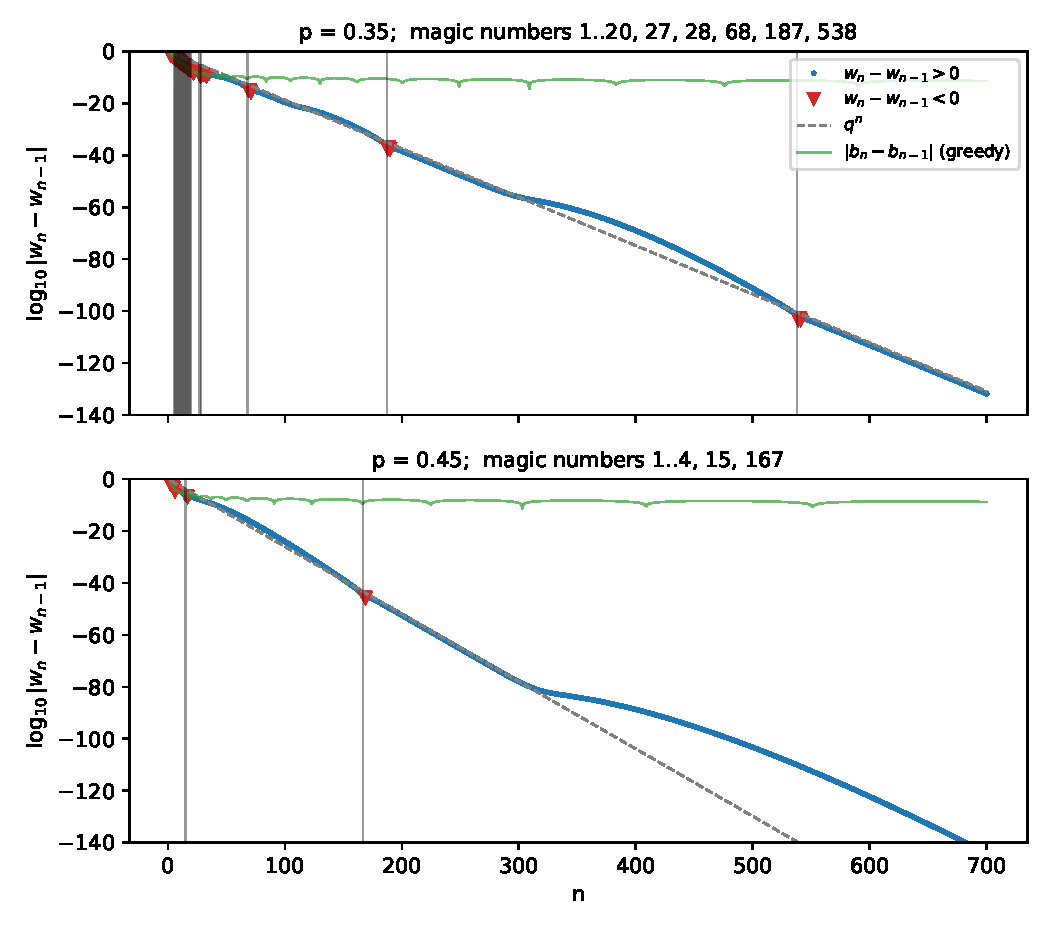
\includegraphics[width=\linewidth]{figures/increments_magic.pdf}
  \caption{Increments $|w_n-w_{n-1}|$ on a logarithmic scale for
    $p=0.35$ (top) and $p=0.45$ (bottom), $n\le700$, computed from the
    exact Bellman recursion in $220$-digit arithmetic.  Red triangles
    mark decreases, vertical lines the magic numbers, the dashed line
    is $q^{n}$, and the green curve is the greedy increment
    $|b_n-b_{n-1}|$, which does not decay.  After each birth the
    increments follow $q^{n}$ (Phase~1), leave that line at
    $n\approx M/q$ (Phase~2), and the next birth occurs when they cross
    it again.}
  \label{fig:increments}
\end{figure}

\subsection{The spacing of magic numbers}\label{sec:ratio}

With Theorem~\ref{thm:magic-inf} the central quantitative question
about the optimal value below the fair coin becomes: \emph{how are the
magic numbers spaced, as a function of $p$?}  We collect what is
proved, what is conjectured, and the numerical evidence.

\paragraph{Upper bound (proved).}  $M_{k+1}<m_1(M_k)$ with
$m_1(M)/M\to C(p)$, the root $r>1$ of $(r-1)\log(q/p)=rH(1/r)$,
$H(x)=-x\log x-(1-x)\log(1-x)$ (Theorem~\ref{thm:magic-inf}).

\paragraph{Lower bound (conditional).}  At a birth after a complete
recovery, the older-record term must decay faster than $q^n$
(Proposition~\ref{prop:ratio} below), which forces
$M_{k+1}+1\ge q(M_k-K)/(1-2p)$ provided the block $(M_k-K,M_k]$
dominates that term (\eqref{eq:geom-lower}).  Note
$q/(1-2p)>1/q$ always, since $1-2p=2q-1$ and $q^2-(2q-1)=p^2>0$: a
birth can only occur after the freeze at $M_k/q$.

\paragraph{The law (conjectured).}  Insert
$\log\gamma_M(\infty)\approx(M/q)\log q$ and $\log\binom{rM}{M}\approx rM\Hent(1/r)$
into the birth criterion~\eqref{eq:birth-approx}; dividing by $M$ the
criterion becomes $g_p(r)>0$ with
\begin{equation}\label{eq:g}
  g_p(r):=(r-1)\log\frac qp\;-\;r\,\Hent(1/r)\;+\;\frac1q\log\frac1q .
\end{equation}
A short computation shows $g_p(1/q)=0$ identically --- the freeze point
is exactly marginal --- and $g_p$ is negative just above $1/q$ and
eventually positive.

\begin{conjecture}[ratio law]\label{conj:ratio}
  For $p\in(0,\tfrac12)$ let $r(p)>1/q$ be the larger root of
  $g_p(r)=0$.  Then $M_{k+1}/M_k\to r(p)$ as $k\to\infty$.
\end{conjecture}

The same number arises from the exact recursion of
Section~\ref{sec:mechanism} without the freeze heuristic: there the
birth is at $n_b=x_bn^*$, $n^*=qM/(1-2p)$, with $J(p,x_b)=I(p)$
in~\eqref{eq:IJ}, and $x_bq/(1-2p)$ coincides with the root of
$g_p$ to all computed digits for every $p$ in Table~\ref{tab:ratio}
(the two equations are the same after the substitution $x=rM$).  The
function $r(p)$ increases from $r(0^+)=1$ to $r(\tfrac12^-)=\infty$;
near $p=\tfrac12$, with $\varepsilon:=\log(q/p)\to0$, the equation reads
$(r-1)\varepsilon\approx\log r-(2\log2-1)$, so
$r(p)\sim\varepsilon^{-1}\log(1/\varepsilon)$.  Always
$q/(1-2p)<r(p)<C(p)$.

\begin{table}[h]
\centering
\small
\begin{tabular}{@{}lrrrl@{}}
\toprule
$p$ & $q/(1-2p)$ & $r(p)$ & $C(p)$ & observed $M_{k+1}/M_k$ (increasing $k$) \\
\midrule
$0.15$ & $1.214$ & $1.255$ & $1.62$ & $1.208,\ 1.209,\ 1.212,\ 1.215,\ 1.218,\ 1.221,\ 1.224,\ 1.227,\ 1.230$ \\
$0.20$ & $1.333$ & $1.426$ & $2.00$ & $1.331,\ 1.345,\ 1.355,\ 1.362,\ 1.372,\ 1.382,\ 1.388,\ 1.395$ \\
$0.25$ & $1.5$   & $1.696$ & $2.56$ & $1.49,\ 1.56,\ 1.59,\ 1.61$ \\
$0.30$ & $1.75$  & $2.155$ & $3.45$ & $1.889,\ 1.971,\ 2.030,\ 2.071,\ 2.099$ \\
$0.35$ & $2.167$ & $3.040$ & $5.07$ & $2.43,\ 2.75,\ 2.88$ \\
$0.40$ & $3.0$   & $5.155$ & $8.63$ & $4.33,\ 4.85$ \\
$0.42$ & $3.625$ & $6.970$ & $11.5$ & $6.35$ \\
$0.45$ & $5.5$   & $13.25$ & $21.0$ & $11.1$ \\
$0.47$ & $8.83$  & $26.46$ & $39.9$ & $24.3$ \\
$0.49$ & $25.5$  & $110.5$ & $151$  & ($M_1=152$) \\
\bottomrule
\end{tabular}
\caption{Spacing of magic numbers: the conditional lower bound
  $q/(1-2p)$, the conjectured limit $r(p)$, the proved upper bound
  $C(p)$, and the observed ratios of consecutive isolated magic
  numbers on the exact trajectories ($n\le2000$ for $p\le0.4$, $n\le700$
  otherwise).  The observed ratios increase with $k$ towards $r(p)$;
  for $p=0.15$ and $0.20$ they cross the lower bound $q/(1-2p)$ around
  the fourth cycle and keep rising, so the slow convergence at small
  $p$ is not a change of law.}\label{tab:ratio}
\end{table}

\paragraph{The two limits.}  As $p\uparrow\tfrac12$ the first
non-trivial magic number escapes to infinity, $M_1(p)\approx\tfrac32/(\tfrac12-p)$
($152$ at $p=0.49$, $27$ at $0.47$, $15$ at $0.45$), and the ratio
$r(p)\to\infty$: on any fixed range of $n$ the sequence looks like the
$p>\tfrac12$ case (decreasing on $\{1,\dots,5\}$, then increasing), which
has no magic numbers at all.  This is why the first-order theory
of~\cite{Paper1}, which works at fixed $n$ as $\tfrac12-p\to0$, sees no
local maximum: the first step of the staircase sits at $n\sim(\tfrac12-p)^{-1}$,
beyond every order of the expansion.  As $p\downarrow0$, $r(p)\to1$ and
the initial stretch on which greedy is optimal and every $n$ is a
record grows without bound ($n_0(p)=69,133,286,690$ for
$p=0.25,0.2,0.15,0.1$).

\paragraph{Relation to Conjecture~\ref{conj:B}.}  Theorem~\ref{thm:magic-inf}
leaves two possibilities for the long-run behaviour: either the
records are eventually isolated and geometrically spaced, with $w$
increasing between the runs of decreases that follow each birth ---
the \emph{staircase} of Example~\ref{ex:policy}, in which the optimal
player plays \One{} except for one \All{} move per cycle at
$n\approx M_k/q$ that lands exactly on $M_k$ --- or from some point on
every index is a record and $w$ is non-increasing forever, in which
case the optimal policy is \All{}.  Conjecture~\ref{conj:B} says the
first alternative holds for every $p<\tfrac12$; Theorem~\ref{thm:notail}
below excludes the second unless the tail starts within a factor
$q^2/(1-2p)$ of the previous record.

%% =====================================================================
\section{Rigorous elements of the cycle theory}\label{sec:cycle}
%% =====================================================================

This section isolates what can be proved about one cycle directly from
the increment identity~\eqref{eq:E}.  Throughout, $M'<M$ are
consecutive magic numbers, and for $n>M$ we write
\[
  \gamma(n):=w_M-w_{n-1}\ (\ge0),\qquad
  x_j:=\max_{j\le m\le M}w_m\ (1\le j\le M),\qquad
  s_n:=\sum_{j=1}^{M'}\omega_{n,j}\,(x_j-w_{n-1})\ (\ge0),
\]
\[
  U_n:=\Prob(\Bin(n,q)\le M'),\qquad V_n:=\Prob(\Bin(n,q)>M),
\]
so that $\gamma(M+1)=0$, $s_n$ is the \emph{older-record term}, and
$U_n$, $V_n$ are exponentially small for $M'/q\ll n\ll M/q$
(the mean $nq$ of the binomial lies between $M'$ and $M$).

\begin{lemma}[exact cycle identity]\label{lem:cycle}
  For every $n>M$ there is $\theta_n\in[0,1]$ such that
  \begin{equation}\label{eq:cycle}
    \gamma(n+1)=\bigl(U_n+V_n-\theta_n(V_n-q^n)\bigr)\gamma(n)
      +q^nw_{n-1}-p^n(1-w_{n-1})-s_n .
  \end{equation}
  Moreover $\theta_n=0$ whenever $w_{n-1}\ge w_j$ for all $M<j<n$
  (in particular whenever $w$ is non-decreasing on $[M+1,n-1]$), and
  $\theta_n\le1$ always.  Consequently, for every $n>M$,
  \begin{equation}\label{eq:cycle-bounds}
    (U_n+q^n)\gamma(n)\;\le\;
    \gamma(n+1)-\bigl[q^nw_{n-1}-p^n(1-w_{n-1})-s_n\bigr]
    \;\le\;(U_n+V_n)\gamma(n).
  \end{equation}
\end{lemma}

\begin{proof}
  Split the sum in~\eqref{eq:E} according to $j\le M'$, $M'<j\le M$,
  $M<j\le n-1$.  For $j\le M'$, $K^{(n)}_j=x_j$ since
  $w_{M'}>w_k$ for all $k>M'$; this gives $s_n$.  For $M'<j\le M$,
  $K^{(n)}_j=w_M$ (every value in $(M',M)$ is below $w_M$, otherwise
  its position would be a record between $M'$ and $M$, and every value
  after $M$ is below $w_M$); these terms contribute
  $\Prob(M'<\Bin(n,q)\le M)\,\gamma(n)=(1-U_n-V_n)\gamma(n)$.  For
  $M<j\le n-1$ the terms $Q_n:=\sum_{j=M+1}^{n-1}\omega_{n,j}
  (K^{(n)}_j-w_{n-1})$ satisfy $0\le Q_n\le(V_n-q^n)\gamma(n)$, because
  $w_{n-1}\le K^{(n)}_j\le w_M$ and the weights sum to
  $\Prob(M<\Bin(n,q)\le n-1)=V_n-q^n$; put
  $\theta_n:=Q_n/((V_n-q^n)\gamma(n))$.  Then
  $\gamma(n+1)=\gamma(n)-d_n$ is~\eqref{eq:cycle}.  If
  $w_{n-1}\ge w_j$ on $(M,n)$ then $K^{(n)}_j=w_{n-1}$ for $j>M$ and
  $Q_n=0$.
\end{proof}

Lemma~\ref{lem:cycle} says that, up to the exponentially small
coefficient of $\gamma(n)$, the gap to the last record is
\emph{memoryless}: $\gamma(n+1)\approx q^nw_{n-1}-s_n$, the all-tails
term minus the older-record term.  This is the rigorous form of
Phase~1.  Three consequences are immediate.

\begin{corollary}[dip criterion]\label{cor:dip}
  For $n>M$: if $q^nw_{n-1}-p^n(1-w_{n-1})-s_n>(1-U_n-q^n)\gamma(n)$
  then $w_n<w_{n-1}$; if $w_n<w_{n-1}$ then
  $q^nw_{n-1}-p^n(1-w_{n-1})-s_n>(1-U_n-V_n)\gamma(n)$.  In particular
  the first dip after $M$ has size $\gamma(M+2)=q^{M+1}w_M-p^{M+1}(1-w_M)-s_{M+1}$
  exactly, and defining the \emph{marginality}
  $m:=s_{M+1}/(q^{M+1}w_M)\in(0,1)$, the run of dips following the birth
  continues at $n$ as long as
  $q^nw_{n-1}-s_n>(1-\varepsilon_n)(q^{n-1}w_{n-2}-s_{n-1})$ with
  $\varepsilon_n\le U_n+V_n$, i.e.\ essentially as long as
  $s_{n-1}-s_n>(1-q)\,q^{n-1}w$: the older-record term must drop by more
  than the all-tails term does.
\end{corollary}

\begin{proof}
  $w_n<w_{n-1}$ iff $\gamma(n+1)>\gamma(n)$; apply~\eqref{eq:cycle-bounds}.
\end{proof}

\begin{lemma}[older-record term]\label{lem:older}
  For $n>M$, with $\rho^+_n:=p(n+1)/(n+1-M')$ and $U'_n:=U_n-p^n$,
  \[
    p\,\bigl(s_n-d_nU'_n\bigr)\;\le\;s_{n+1}\;\le\;\rho^+_n\bigl(s_n-d_nU'_n\bigr).
  \]
  In particular $s_{n+1}\le\rho^+_n s_n$ whenever $d_n\ge0$.
\end{lemma}

\begin{proof}
  $\omega_{n+1,j}=\omega_{n,j}\,p(n+1)/(n+1-j)$ and
  $p\le p(n+1)/(n+1-j)\le\rho^+_n$ for $1\le j\le M'$; and
  $x_j-w_n=(x_j-w_{n-1})-d_n$, with $\sum_{j\le M'}\omega_{n,j}=U'_n$.
\end{proof}

\begin{proposition}[freeze bound]\label{prop:freeze}
  Let $n_1:=\max\{n>M:\ U_k+V_k\le\tfrac12\text{ for }M<k\le n\}$.  Then
  $\gamma(n)\le C_qq^{\,n-1}$ for $M<n\le n_1+1$, $C_q:=2q/(2q-1)$, and
  \[
    0\;\le\;w_M-W(p)\;\le\;C_qq^{\,n_1}+q^{\,n_1+1}/p .
  \]
  Since $V_n\le\tfrac14$ for $n\le(M-c\sqrt{M\log M})/q$ and
  $U_n\le\tfrac14$ for $n\ge M$ (Chernoff), $n_1\ge(M-c\sqrt{M\log M})/q$
  and hence $w_M-W(p)\le C\,q^{(M-c\sqrt{M\log M})/q}$.
\end{proposition}

\begin{proof}
  By~\eqref{eq:cycle-bounds}, $\gamma(n+1)\le q^n+\tfrac12\gamma(n)$ for
  $M<n\le n_1$; induction from $\gamma(M+1)=0$ gives
  $\gamma(n)\le C_qq^{n-1}$ (the constant satisfies
  $1+C_q/(2q)=C_q$).  Finally $w_{n-1}-W(p)\le\sum_{i\ge n}d_i^-\le q^n/p$
  by Theorem~\ref{thm:conv}, so $w_M-W(p)\le\gamma(n)+q^n/p$.
\end{proof}

\begin{proposition}[the older-record term must decay faster than $q$ at a birth]\label{prop:ratio}
  Suppose $w_{M-1}\ge w_j$ for all $M'<j<M$ (complete recovery before
  the birth).  Then
  \[
    s_M\;\ge\;q^Mw_{M-1}-p^M(1-w_{M-1}),\qquad
    s_{M+1}\;<\;q^{M+1}w_M-p^{M+1}(1-w_M),
  \]
  hence
  \[
    \frac{s_{M+1}}{s_M}\;<\;q\cdot\frac{w_M}{w_{M-1}}\cdot
    \Bigl(1-\frac{(p/q)^M(1-w_{M-1})}{w_{M-1}}\Bigr)^{-1}
    \;=\;q\,\bigl(1+O(q^{M'}/p+(p/q)^M)\bigr),
  \]
  using $0\le d_M\le\sum_{i>M'}d_i^-\le q^{M'+1}/p$.
\end{proposition}

\begin{proof}
  $M-1$ is not a record and $M$ is, so $d_M\ge0$ and $d_{M+1}<0$.
  Evaluate~\eqref{eq:E} at $n=M$ (where, by the hypothesis, the terms
  with $M'<j<M$ vanish and those with $j\le M'$ give $s_M$) and at
  $n=M+1$ (where $\gamma(M+1)=0$ and there are no terms with $j>M$).
\end{proof}

Proposition~\ref{prop:ratio} is the rigorous core of the ratio law.
Since the weights $\omega_{n,j}$, $j\le M'$, are concentrated near
$j=M'$ and $\omega_{n+1,j}/\omega_{n,j}=p(n+1)/(n+1-j)$, the ratio
$s_{M+1}/s_M$ is $p(M+1)/(M+1-M')\,(1+o(1))$ provided the block
$(M'-K,M']$ with $K=O(\log M)$ carries most of $s_M$; then the
proposition forces
\begin{equation}\label{eq:geom-lower}
  M+1\;\ge\;\frac{q}{1-2p}\,(M'-K)\,(1-o(1)),
\end{equation}
a rigorous \emph{geometric lower bound} on the growth of magic numbers,
with the same ratio $q/(1-2p)$ at which the older-record term stops
decaying faster than $q^n$ in Lemma~\ref{lem:older}.  Note that
$q/(1-2p)>1/q$ always, since $1-2p=2q-1$ and $q^2-(2q-1)=(1-q)^2=p^2>0$;
so a birth can only occur after the freeze, and
$q/(1-2p)<r(p)$ for all $p$ (Table~\ref{tab:ratio}); the observed
ratios cross $q/(1-2p)$ after a few cycles and continue towards
$r(p)$.  The block-domination
hypothesis is where the proof of~\eqref{eq:geom-lower} is still open;
the theorem below shows what it, together with the exact identity,
yields for one full cycle, and how the estimates propagate from one
cycle to the next.

\subsection{The mechanism of a cycle}\label{sec:mechanism}

\begin{conjecture}[cycle structure]\label{conj:cycle}
  For every $p\in(0,\tfrac12)$ and every $k$ large enough, the magic
  numbers of Theorem~\ref{thm:magic-inf} satisfy
  $M_{k+1}+1\ge(1+c)\,qM_k/(1-2p)$ for some fixed $c>0$, the run of
  decreases after $M_k$ is bounded, and $w$ increases from its end to
  the birth of $M_{k+1}$.
\end{conjecture}

Two exact facts turn the transition between the memoryless Phase~1
and the next birth into a one-dimensional recursion.  Write
$P_n:=1-U_n-V_n=\Prob(M'<\Bin(n,q)\le M)$.

\begin{lemma}[when the binomial tail decays slower than $q^n$]\label{lem:tailratio}
  Let $\tau_n:=\Prob(\Bin(n,q)\le M)$ and $n^*:=qM/(1-2p)$.  Then
  $\tau_{n+1}/\tau_n=1-q\,\Prob(\Bin(n,q)=M)/\tau_n$, and with
  $\kappa_n:=Mp/((n+1-M)q)$ the ratio of the two top terms of $\tau_n$,
  \[
    \frac{\tau_{n+1}}{\tau_n}\ \ge\ q \quad\text{if}\quad
    \frac{\kappa_n}{1-\kappa_n}\Bigl(1-O\bigl(\tfrac{\log M}{M}\bigr)\Bigr)\ge\frac{1-2p}{p},
    \qquad
    \frac{\tau_{n+1}}{\tau_n}\ \le\ p+q\kappa_n .
  \]
  Since $\kappa_n/(1-\kappa_n)\ge(1-2p)/p$ iff $\kappa_n\ge(1-2p)/q$ iff
  $n+1\le n^*$, the tail $\tau_n/q^n$ increases up to
  $n=n^*(1-O(\log M/M))$ and decreases geometrically afterwards.  In
  particular $\rho^+_n=p(n+1)/(n+1-M')\le\lambda q$ with
  $\lambda=p(1+c)/(p+cq)<1$ whenever $n+1\ge(1+c)qM'/(1-2p)$.
\end{lemma}

\begin{proof}
  The identity is $\Prob(\Bin(n+1,q)\le M)=\tau_n-q\Prob(\Bin(n,q)=M)$.
  Write $\tau_n/\Prob(\Bin(n,q)=M)=\sum_{i\ge0}\prod_{l<i}\kappa^{(l)}_n$
  with $\kappa^{(l)}_n=(M-l)p/((n+1-M+l)q)$ decreasing in $l$ from
  $\kappa_n$; truncating at $i=K=O(\log M)$ gives
  $\ge1+\kappa_n/(1-\kappa_n)-O(K/M)$, and $1/(1-\kappa_n)$ is an upper
  bound; then $\tau_{n+1}/\tau_n\ge q$ iff $\tau_n/\Prob(\Bin=M)\ge q/p$.
  The last claim: $p(n+1)/(q(n+1-M'))$ at $n+1=(1+c)qM'/(1-2p)$ equals
  $p(1+c)/(p+cq)$ (use $1-2p=2q-1$), and it decreases in~$n$.
\end{proof}

\begin{lemma}[the normalised gap]\label{lem:A}
  For $n>M$ put $\varepsilon_n:=\sigma_n+(p/q)^n(1-w_{n-1})/w_{n-1}$ and
  $A_n:=\gamma(n)P_n/(q^nw_{n-1})$.  Then $d_n\ge0$ iff
  $A_n\ge1-\varepsilon_n$, and whenever $\theta_n=0$,
  \begin{equation}\label{eq:Arec}
    A_{n+1}=\frac{P_{n+1}}{q\,P_n}\cdot\frac{w_{n-1}}{w_n}\cdot
    \bigl[(1-P_n)A_n+P_n(1-\varepsilon_n)\bigr].
  \end{equation}
\end{lemma}

\begin{proof}
  With $\theta_n=0$, \eqref{eq:cycle} reads
  $\gamma(n+1)=(1-P_n)\gamma(n)+q^nw_{n-1}(1-\sigma_n)-p^n(1-w_{n-1})$ and
  $d_n=\gamma(n)-\gamma(n+1)=q^nw_{n-1}[A_n+\varepsilon_n-1]$.
\end{proof}

Lemma~\ref{lem:A} says that the increase after a birth persists
exactly as long as $A_n\ge1-\varepsilon_n$, with $\varepsilon_n$
exponentially small after the run, and that $A$ evolves by an
explicit recursion whose only $n$-dependent input is the tail ratio
of Lemma~\ref{lem:tailratio}: in the flat range $A_{n+1}\approx1/q>1$;
through the transition $A$ is multiplied by $\tau_{n+1}/(q\tau_n)$,
which is $\ge1$ up to $n^*$ and $<1$ beyond.  Thus $\log A$ gains
$\approx MI(p)$ up to $n^*$ and then loses $\approx MJ(p,n/n^*)$,
\begin{equation}\label{eq:IJ}
  I(p):=\int_{1/q}^{q/(1-2p)}\log\frac{px}{q(x-1)}\,dx,\qquad
  J(p,x):=\int_{q/(1-2p)}^{xq/(1-2p)}\log\frac{q(x'-1)}{px'}\,dx' ,
\end{equation}
and the next birth is where $A$ returns to $1$: $n_b=x_bn^*$ with
$J(p,x_b)=I(p)$.  For $p=0.45$: $I=0.6178$, $x_b=2.409$,
$n_b/M=x_bq/(1-2p)=13.251$, exactly the root $r(p)$ of
Conjecture~\ref{conj:ratio} --- the ratio law derived from the exact
recursion.  On the exact trajectories the criterion
$d_n\ge0\iff A_n\ge1-\varepsilon_n$ holds at every $n$ of every cycle;
e.g.\ $p=0.25$, $M=292$: $A=1.52$ at $M/q$, $14.1$ at $n^*=438$,
$1.036$ at $471$ and $0.900$ at the birth $472$.  What this does
\emph{not} give is a proof: to run~\eqref{eq:Arec} one needs the run
after $M$ to end and $\sigma$ to decay, which needs the position of
$M$ relative to $M'$ --- Conjecture~\ref{conj:cycle} is exactly the
statement that this regularity propagates from cycle to cycle, and
the previous version of this section proved that it does, under an
explicit growth hypothesis and for $M$ beyond an unspecified
$M_0(p)$; we do not reproduce that induction here.

\subsection{A non-increasing tail cannot start late}\label{sec:notail}

We now argue by contradiction.  Suppose Conjecture~\ref{conj:B} fails:
$w$ is non-increasing on $[N,\infty)$, with $N$ minimal, so that
$w_{N-1}<w_N$ and $N$ is a record.  Let $M'<N$ be the last strict
record before $N$, and use the notation of Lemma~\ref{lem:cycle} with
$M$ replaced by $N$: $\gamma(n)=w_N-w_{n-1}$ (now non-decreasing in
$n$), $s_n$, $\sigma_n=s_n/(q^nw_{n-1})$, $P_n=\Prob(M'<\Bin(n,q)\le N)$.
Since $d_n\le0$ for all $n>N$, \eqref{eq:E} gives for all $n>N$
\begin{equation}\label{eq:tailI}
  q^nw_{n-1}\ \ge\ p^n(1-w_{n-1})+s_n+P_n\gamma(n)+Q_n ,
  \qquad Q_n=\sum_{j=N+1}^{n-1}\omega_{n,j}(w_j-w_{n-1})\ge0 .
\end{equation}

\begin{theorem}[no late tails]\label{thm:notail}
  Fix $c>0$ and put $\lambda_c:=p(1+c)/(p+cq)<1$.  There is
  $N_0(p,c)$ such that a non-increasing tail as above with
  $N+1\ge(1+c)\,qM'/(1-2p)$ has $N\le N_0(p,c)$.
\end{theorem}

\begin{proof}
  \emph{Flatness.}  Let $n_1:=\max\{n:P_n\ge\tfrac12\}$; by Chernoff,
  $n_1\ge(N-C\sqrt{N\log N})/q$.  From~\eqref{eq:tailI},
  $P_n\gamma(n)\le q^n$, and $\gamma$ is non-decreasing, so
  $\gamma(n)\le\gamma(n_1)\le2q^{n_1}$ for all $n\le n_1$.

  \emph{Tracking.}  For $N<k\le n_1$, \eqref{eq:tailI} rewritten reads
  $0\le-d_k=q^kw_{k-1}(1-\sigma_k)-p^k(1-w_{k-1})-P_k\gamma(k)-Q_k$,
  so $\sigma_k\le1$, and $\sum_{k=N+1}^{n_1}(-d_k)=\gamma(n_1+1)\le2q^{n_1}$.
  Since $P_k\gamma(k)+Q_k\le\gamma(k)\le2q^{n_1}$, each summand
  satisfies $q^kw_{k-1}(1-\sigma_k)\le2q^{n_1}(1+2n_1)+p^k$, i.e.
  \[
    1-\eta_k\ \le\ \sigma_k\ \le\ 1,\qquad
    \eta_k:=\frac{2(1+2n_1)q^{\,n_1-k}+(p/q)^k}{a_\infty},
    \qquad N<k\le n_1 .
  \]
  Thus $s_{k+1}/s_k=q\,(w_k/w_{k-1})\,\sigma_{k+1}/\sigma_k\ge q(1-\eta_{k+1})(1-q^k/a_\infty)$:
  \emph{the older-record term must track $q^kw$ exactly}, up to
  exponentially small errors, on the window $(N,n_1]$.

  \emph{Decay.}  By Lemma~\ref{lem:older}, $s_{k+1}\le\rho^+_k(s_k+|d_k|U'_k)$
  with $\rho^+_k=p(k+1)/(k+1-M')$, and $|d_k|U'_k/s_k\le q^kU'_k/(q^kw(1-\eta_k))\le2U'_k/a_\infty$,
  where $U'_k=\Prob(\Bin(k,q)\le M')$ is exponentially small for
  $k\ge N$ because $Nq\ge(1+c)q^2M'/(1-2p)>M'$.  The hypothesis
  $N+1\ge(1+c)qM'/(1-2p)$ gives $\rho^+_k\le\lambda_cq$ for $k\ge N$
  (the same computation as in Lemma~\ref{lem:tailratio}).  Hence
  $s_{k+1}/s_k\le\lambda_cq(1+2U'_k/a_\infty)$, which contradicts the
  tracking bound as soon as $\eta_{k+1}+q^k/a_\infty+2U'_k/a_\infty<1-\lambda_c$,
  i.e.\ for $N$ large.
\end{proof}

The proof is uniform in $p$ and uses nothing beyond~\eqref{eq:E}.
The same three steps give a conditional form of the gap bound that
Section~\ref{sec:magic} needs.

\begin{proposition}[gap bound, conditional]\label{prop:gap}
  Let $M'<M$ be consecutive records and suppose that after the run
  following $M$ the sequence is non-decreasing, with
  $w_{n-1}\ge\max_{M<j<n}w_j$, up to the next decrease at $n_b$
  (Phase~1 and Phase~2 without intermediate dips), and that
  $\sigma_k\le\tfrac12$ for $k\ge k_1$ and $n_b>k_1+1$, where
  $k_1\ge M/q+C\sqrt{M\log M}$ is such that $\sum_{i>k_1}\Prob(\Bin(i,q)\le M)\le1$.
  Then
  \[
    w_M-W(p)\ \ge\ w_M-w_{n_b-1}\ \ge\ \frac{a_\infty}{4e^{2}}\,q^{\,k_1}.
  \]
\end{proposition}

\begin{proof}
  With $\theta_n=0$, \eqref{eq:cycle} gives
  $\gamma(n+1)=(1-P_n)\gamma(n)+q^nw_{n-1}(1-\sigma_n)-p^n(1-w_{n-1})
  \ge V_n\gamma(n)+q^na_\infty/4$ for $k_1\le n<n_b$; iterate and keep the
  first summand: $\gamma(n_b)\ge\tfrac{a_\infty}4q^{k_1}\prod_{i>k_1}V_i
  \ge\tfrac{a_\infty}{4e^2}q^{k_1}$, as $\log(1-x)\ge-2x$ for $x\le\tfrac12$.
  Finally $W(p)\le w_{n_b-1}$ because $n_b-1$ is a record: the increase
  phase leaves every later value below $w_{n_b-1}$ by the same
  computation, since $\tilde\sigma$ decays after $n_b$ (Lemma~\ref{lem:older}).
\end{proof}

The hypothesis of Proposition~\ref{prop:gap} is the regularity of the
cycle after~$M$, and the only way we know to guarantee it is the
growth condition $M+1\ge(1+c)qM'/(1-2p)$ for the pair before
(then $\sigma$ decays geometrically by Lemma~\ref{lem:older}, the run
is bounded, and Lemma~\ref{lem:A} carries the increase past~$k_1$).
So the gap bound for $M$ rests on the position of $M$ relative to
$M'$, which rests on the cycle before --- the induction of the
previous version of this section.  We do not know how to break this
chain from below; Theorem~\ref{thm:notail} shows what can be said
without it: a counterexample to Conjecture~\ref{conj:B} would have to
be an \emph{early} tail, $N+1<(1+c)qM'/(1-2p)$.

\subsection{Tracking forces dense records}\label{sec:tracking}

The tracking step of Theorem~\ref{thm:notail} is a statement about
non-negative combinations of binomial weights, and it has a sharp
converse: a combination $\sum_{j\le J}c_j\omega_{k,j}$ with $c_j\ge0$
can behave like $Aq^k$ on a long window of $k$ only if its mass is
concentrated, for every $k$, near a specific moving index.

\begin{lemma}[tilting]\label{lem:tilting}
  Let $c_j\ge0$ ($0\le j\le J$), $S_k:=\sum_{j\le J}c_j\omega_{k,j}$,
  and $r_{k,j}:=\omega_{k+1,j}/\omega_{k,j}=p(k+1)/(k+1-j)$.  Let
  $\mu_k(j):=c_j\omega_{k,j}/S_k$.  Then $S_{k+1}/S_k=\mathbb E_{\mu_k}[r_{k,\cdot}]$,
  $\mu_{k+1}(j)=\mu_k(j)\,r_{k,j}/\mathbb E_{\mu_k}[r_{k,\cdot}]$, and
  \[
    \frac{S_{k+2}}{S_{k+1}}
    \ \ge\ \Bigl(\frac{S_{k+1}}{S_k}+\frac{\operatorname{Var}_{\mu_k}(r_{k,\cdot})}{S_{k+1}/S_k}\Bigr)
    \Bigl(1-\frac{J}{(k+1)(k+2-J)}\Bigr).
  \]
\end{lemma}

\begin{proof}
  The first two identities are $\omega_{k+1,j}=\omega_{k,j}r_{k,j}$.
  Then $\mathbb E_{\mu_{k+1}}[r_{k,\cdot}]=\mathbb E_{\mu_k}[r_{k,\cdot}^2]/\mathbb E_{\mu_k}[r_{k,\cdot}]
  =m_k+\operatorname{Var}_{\mu_k}(r_{k,\cdot})/m_k$ with $m_k=S_{k+1}/S_k$,
  and $r_{k+1,j}=r_{k,j}\bigl(1-j/((k+1)(k+2-j))\bigr)\ge r_{k,j}(1-J/((k+1)(k+2-J)))$.
\end{proof}

\begin{proposition}[concentration]\label{prop:concentration}
  Suppose $S_k=Aq^k(1+\eta_k)$ with $|\eta_k|\le\eta$ for all $k$ in a
  window $[K_1,K_2]$ with $K_1\ge J/q$.  Then for every $k\in[K_1,K_2-1]$,
  \[
    \operatorname{Var}_{\mu_k}(j)\ \le\ \Bigl(\frac qp\Bigr)^{2}\Bigl(4\eta k^2+\frac{J}{p}\Bigr)
    \qquad\text{and}\qquad
    \mathbb E_{\mu_k}[j]=j^*(k)+O\bigl(\eta k+J/k\bigr),
    \quad j^*(k):=(k+1)\Bigl(1-\frac pq\Bigr).
  \]
  In words: the measure $c_j\omega_{k,j}$ is concentrated within
  $O(\sqrt{J}+k\sqrt\eta)$ of $j^*(k)$, and $j^*(k)$ sweeps the interval
  $[(1-p/q)K_1,(1-p/q)K_2]$ as $k$ runs through the window.
\end{proposition}

\begin{proof}
  Tracking gives $m_k,m_{k+1}\in[q(1-2\eta),q(1+2\eta)]$, so
  Lemma~\ref{lem:tilting} yields
  $\operatorname{Var}_{\mu_k}(r)\le m_k\bigl(m_{k+1}/(1-\varepsilon_k)-m_k\bigr)
  \le q^2(4\eta+\varepsilon_k)(1+O(\eta))$ with
  $\varepsilon_k=J/((k+1)(k+2-J))\le J/(p(k+1)^2)$ for $k\ge J/q$.
  Since $j\mapsto r_{k,j}$ is increasing with $\partial_jr_{k,j}\ge p/(k+1)$,
  $\operatorname{Var}(r)\ge(p/(k+1))^2\operatorname{Var}(j)$ (pair formula for the
  variance), which is the first claim.  For the second, $r_{k,\cdot}$
  is convex, so $r_{k,\mathbb E j}\le\mathbb E[r]=m_k$ (Jensen) gives
  $\mathbb Ej\le j^*(k)(1+O(\eta))$; and
  $\mathbb E[r]\le r_{k,\mathbb Ej}+\tfrac12\max r''\operatorname{Var}(j)$ with
  $r''\le2p(k+1)/(k+1-J)^3$ gives $\mathbb Ej\ge j^*(k)-O(\eta k+J/k)$,
  using $r_{k,j}=q\iff j=j^*(k)$.
\end{proof}

\begin{corollary}[dense records]\label{cor:dense}
  In the situation of Theorem~\ref{thm:notail} (a non-increasing tail
  from $N$, previous record $M'$), apply
  Proposition~\ref{prop:concentration} to $c_j=x_j-w$ ($j\le J=M'$),
  which is constant on the blocks between consecutive records below
  $M'$, on the window $(N,n_1-C\log N]$, where the tracking error
  $\eta$ is exponentially small.  Within a block $(M_i,M_{i+1}]$ the
  weight $\omega_{k,j}$ grows geometrically in $j$ (ratio
  $\ge q/(q-p)$ near $j^*(k)$), so $\mu_k$ restricted to a block is
  concentrated at its right end, the record $M_{i+1}$.  Hence:
  \emph{for every $k$ in the window there is a record within
  $O(\sqrt{M'})$ of $j^*(k)$}, i.e.\ the records are
  $O(\sqrt{M'})$-dense on the interval
  $[(1-p/q)(N+2),\,(1-p/q)(n_1-C\log N)]$, and in particular
  $(1-p/q)n_1\le M'+O(\sqrt{M'})$, i.e.
  \[
    N\ \le\ \frac{q^{2}}{1-2p}\,M'\,\bigl(1+o(1)\bigr)
  \]
  --- a counterexample tail must start within a factor $q^2/(1-2p)$
  of the previous record, and it must be preceded by a stretch of
  relative length $\ge1/q$ on which records are dense, that is, on
  which $w$ is non-increasing up to fluctuations of size $q^{n}$.
\end{corollary}

\begin{remark}[descent]
  Corollary~\ref{cor:dense} replaces the tail on $[N,\infty)$ by a
  quasi-tail (dense records) on $[(1-p/q)N,M']$, one scale factor
  $1-p/q$ below.  If the tracking argument can be run on a
  quasi-tail --- the missing piece is that between dense records $w$
  is not exactly non-increasing, so~\eqref{eq:tailI} holds only up to
  the small increases $d_n^+$ --- the descent continues to scales
  $(1-p/q)^kN$, and it must stop at scales of order one, where the
  sequence is known explicitly ($w$ is strictly decreasing on
  $\{1,\dots,5\}$ and $\{1,\dots,n_0(p)\}$ but the records there are
  consecutive, not $O(\sqrt{\cdot})$-dense relative to their scale in
  the required sense once $n\ge 2$).  This would be a proof of
  Conjecture~\ref{conj:B} uniform in $p$, with no computation and no
  induction over cycles.  We have not carried out the quasi-tail step.
\end{remark}

%% =====================================================================
\section{Numerical evidence}\label{sec:numerics}
%% =====================================================================

All values were computed from the exact Bellman
recursion~\eqref{eq:bellman} in $220$-digit (and, as a check,
$320$-digit) floating-point arithmetic with \texttt{mpmath}; the scripts
\texttt{simulation/magic\_numbers.py} and
\texttt{simulation/magic\_birth.py} in the repository~\cite{Repo}
reproduce every number below.  The identity~\eqref{eq:E} was verified
to $10^{-220}$ for all $n\le700$ and all $p$ in Table~\ref{tab:grid}.

\begin{table}[h]
\centering
\footnotesize
\setlength{\tabcolsep}{4pt}
\begin{tabular}{@{}lllrrr@{}}
\toprule
$p$ & magic numbers on $[1,700]$ & decreases ($n\ge10$) &
 $\mathrm{osc}\,w$ & $\mathrm{osc}\,b$ & $w_{700}-b_{700}$ \\
\midrule
$0.15$ & $1..271,\,313,\,378,\,457,\,554,\,673$ & $10$–$286$, $314$–$325$, \dots & $2\cdot10^{-25}$ & $4\cdot10^{-23}$ & $1\cdot10^{-25}$ \\
$0.20$ & $1..126,\,148,\,197,\,265,\,359,\,489,\,671$ & $10$–$133$, $149$–$160$, \dots & $1\cdot10^{-34}$ & $3\cdot10^{-17}$ & $2\cdot10^{-18}$ \\
$0.25$ & $1..66,\,77,\,78,\,79,\,118,\,184,\,292,\,471$ & $10$–$69$, $78$–$88$, $119$–$122$, \dots & $2\cdot10^{-44}$ & $1\cdot10^{-13}$ & $6\cdot10^{-14}$ \\
$0.30$ & $1..38,\,54,\,102,\,201,\,408$ & $10$–$42$, $55$–$60$, $103$–$105$, \dots & $4\cdot10^{-52}$ & $5\cdot10^{-11}$ & $8\cdot10^{-11}$ \\
$0.35$ & $1..20,\,27,\,28,\,68,\,187,\,538$ & $10$–$22$, $28$–$33$, $69$–$71$, \dots & $1\cdot10^{-60}$ & $3\cdot10^{-9}$ & $1\cdot10^{-8}$ \\
$0.40$ & $1..11,\,24,\,104,\,504$ & $10$–$14$, $25$–$27$, $105$–$107$, $505$–$506$ & $5\cdot10^{-70}$ & $7\cdot10^{-8}$ & $1\cdot10^{-6}$ \\
$0.42$ & $1..6,\,9,\,10,\,43,\,273$ & $10$–$13$, $44$–$45$, $274$–$275$ & $2\cdot10^{-83}$ & $3\cdot10^{-7}$ & $6\cdot10^{-6}$ \\
$0.45$ & $1..4,\,15,\,167$ & $16$–$17$, $168$–$169$ & $1\cdot10^{-83}$ & $9\cdot10^{-7}$ & $2\cdot10^{-4}$ \\
$0.47$ & $1..3,\,27,\,657$ & $28$–$29$, $658$–$659$ & $9\cdot10^{-89}$ & $1\cdot10^{-6}$ & $2\cdot10^{-4}$ \\
$0.49$ & $1..3,\,152$ & $153$–$154$ & $2\cdot10^{-92}$ & $1\cdot10^{-6}$ & $2\cdot10^{-4}$ \\
\bottomrule
\end{tabular}
\caption{Magic numbers, decreases, and relative oscillation
  $\mathrm{osc}\,x:=(\max-\min)/\max$ over $n\in[350,700]$ of the
  optimal value $w$ and the greedy value $b$.  ``$1..k$'' abbreviates
  the initial run $1,2,\dots,k$ of consecutive magic numbers, on which
  greedy is optimal and $w=b$ exactly.}\label{tab:grid}
\end{table}

Three features stand out.  First, $w$ converges while $b$ does not: the
two oscillation columns differ by $10$ to $80$ orders of magnitude.
Second, for small $p$ the greedy strategy is optimal on a long initial
stretch ($w_n=b_n$ exactly for $n\le66$ at $p=0.25$, for $n\le271$ at
$p=0.15$, for $n\le682$ at $p=0.10$), after which isolated magic numbers
appear; this initial run is the regime $\mathcal M_p\supseteq[1,n_0(p)]$
in which $w$ is strictly decreasing, and $n_0(p)\to\infty$ as
$p\to0$.  Third, each birth is followed by a run of two to a dozen
consecutive decreases (the transient of Phase~1: the birth is marginal,
so the first gap $|d_{M+1}|$ is much smaller than $q^{M+1}$, and a few
more decreases are needed before $\gamma(n)\approx q^{n}w$ is
reached), after which $w$ increases until the next birth.  The size of
a decrease relative to the bound~\eqref{eq:dipbound} is small but not
negligible: at $p=0.45$, $-d_{168}/q^{168}\approx0.03$.

The next births beyond $n=700$ can be extrapolated
from~\eqref{eq:birth-approx} with $\gamma_M(\infty)$ replaced by
$w_M-w_{700}$ (an upper bound, so the prediction is an upper bound):
$n\lesssim2140$ for $p=0.45$ and $n\lesssim1843$ for $p=0.42$.

%% =====================================================================
\section{Discussion}\label{sec:discussion}
%% =====================================================================

\paragraph{The greedy gap.}  Since $w\ge b$ and $w$ converges while $b$
oscillates, $w_n-b_n$ oscillates with the amplitude of $b$ around a
positive mean; at $p=0.45$ the mean gap is $1.5\cdot10^{-4}$, at
$p=0.25$ it is $6\cdot10^{-14}$.  Greedy is therefore not asymptotically
optimal, but its loss is a constant, not a growing quantity.  A proof
that $W(p)>\limsup_n b_{n,p}$ for all $p<\tfrac12$ would follow from
the strict inequality $w_{m}>b_{m}$ at the first isolated magic number,
combined with the supersolution property of~$w$.

\paragraph{Status of Conjecture~\ref{conj:B}.}  Suppose $w$ were
eventually non-increasing, from $M$ on.  Then $K^{(n)}_j=w_j$ for
$j\ge M$, so beyond $M$ the value satisfies the \emph{greedy} recursion
with modified data, and the analysis of~\cite{Paper2} applies: $w$ has a
log-periodic profile, which by Theorem~\ref{thm:conv} must be
constant.  This was the reduction of our earlier approach (its
``Gap~D''); it asks for non-cancellation, and we now know that
cancellation is precisely what the optimal player achieves whenever a
magic number is available.  What is needed instead is an argument that
a non-increasing tail cannot be self-consistent: from~\eqref{eq:E},
$d_n\le0$ for all $n>M$ forces
$\sum_{j\ge M}\omega_{n,j}(w_j-w_{n-1})\le q^{n}$, i.e.\ the binomial
average of the decrements at scale $nq$ is at most $q^{n}$, which after
iteration bounds $w_n-W(p)$ by $O(q^{n/q})$; a coupling of the games
with $n$ and $n+1$ coins gives complementary bounds.  We have not
closed this gap.  We note that the conjecture is the exact analogue of
van~Doorn's ``infinitely complex'' conjecture~\cite[\S10]{vanDoorn} for
the all-heads objective: the answer to ``with two tails, keep two coins
or three?'' changes infinitely often iff the set of magic numbers is
infinite.

\paragraph{The amplitude functional.}  The conjecture can be made
quantitative.  Fix a magic number $M$ and let $z=z^{(M)}$ be the
\emph{forced greedy continuation}: $z_n=w_n$ for $n\le M$ and
$z_n=\sum_{j=0}^{n-1}\omega_{n,j}x_j$ for $n>M$, with $x_0=1$,
$x_j=\max_{j\le m\le M}w_m$ for $1\le j\le M$ and $x_j=z_j$ for $j>M$.
This is what $w$ would be if it were non-increasing from $M$ on, so
Conjecture~\ref{conj:B} says: \emph{no $z^{(M)}$ is eventually
non-increasing.}  Poissonising, $Z(t):=\mathbb E[z_{\mathrm{Po}(t)}]$
satisfies the exact functional equation
$Z(t)=(1-e^{-pt})Z(qt)+S(t)$ with
$S(t)=(1-e^{-pt})e^{-qt}P(qt)+e^{-t}R(t)$, where
$P(u)=\sum_{j\le M}(x_j-w_j)u^j/j!$ and $R(u)=\sum_{n\le M}r_nu^n/n!$,
$r_n=w_n-\sum_{j<n}\omega_{n,j}x_j$, are polynomials determined by the
data up to~$M$.  Iterating, $Z(t)=\sum_{k\ge0}\prod_{i<k}(1-e^{-pq^it})
S(q^kt)$, and exactly as in~\cite{Paper2} one obtains
$Z(t)=\Phi_M(\log t)+O(e^{-ct})$ with the $L$-periodic profile
$\Phi_M(\tau)=\sum_{k\in\mathbb Z}\Pi(q^ke^\tau)S(q^ke^\tau)$,
$\Pi(u)=\prod_{j\ge1}(1-e^{-pu/q^j})$, whose Fourier coefficients are
\begin{equation}\label{eq:amplitude}
  A_m(M)=\frac1L\int_0^\infty u^{2\pi im/L-1}\,\Pi(u)\,S(u)\,du .
\end{equation}
If $A_1(M)\ne0$, the profile is non-constant, and after analytic
de-Poissonisation (with error relative to the oscillation, since the
kernel is linear) $z^{(M)}$ oscillates and is not eventually monotone:
Conjecture~\ref{conj:B} holds at~$M$.  Thus
\[
  \text{Conjecture~\ref{conj:B}}\iff A_1(M)\ne0\ \text{for every magic
  number } M .
\]
Formula~\eqref{eq:amplitude} is explicit and was evaluated numerically
(\texttt{simulation/continuation\_amplitude.py}).  Validation: for
$M=0$ (pure greedy) $A_0$ reproduces the mean of $b_n$ to ten digits
and $4|A_1|$ its peak-to-peak oscillation ($p=0.45$: $3.4\cdot10^{-7}$
vs.\ $3.8\cdot10^{-7}$ on $n\in[350,700]$); for $p=0.45$, $M=15$, a
direct computation of $z^{(15)}$ up to $n=3000$ gives mean
$0.411292054$ and peak-to-peak $3.34\cdot10^{-8}$, against
$A_0=0.411292054$ and $4|A_1|=3.24\cdot10^{-8}$ --- and $z^{(15)}$
indeed changes direction $11$ times on $[100,3000]$.  At the magic
numbers:
\begin{center}
\begin{tabular}{@{}lrrrr@{}}
\toprule
$p$ & $M$ & $|A_1(M)|$ & $|A_2(M)|$ & $|A_1(M)|/q^M$ \\
\midrule
$0.45$ & $15$  & $8.1\cdot10^{-9}$  & $8\cdot10^{-13}$ & $6\cdot10^{-5}$ \\
$0.45$ & $167$ & $2.8\cdot10^{-47}$ & $1\cdot10^{-47}$ & $6.4\cdot10^{-4}$ \\
$0.25$ & $79$  & $1.1\cdot10^{-15}$ & $3\cdot10^{-20}$ & $8\cdot10^{-6}$ \\
$0.25$ & $118$ & $3.4\cdot10^{-19}$ & $6\cdot10^{-22}$ & $1.9\cdot10^{-4}$ \\
$0.25$ & $184$ & $3.0\cdot10^{-27}$ & $5\cdot10^{-29}$ & $3.0\cdot10^{-4}$ \\
$0.25$ & $292$ & $1.1\cdot10^{-40}$ & $9\cdot10^{-42}$ & $3.6\cdot10^{-4}$ \\
$0.25$ & $471$ & $5.0\cdot10^{-63}$ & $1\cdot10^{-63}$ & $3.3\cdot10^{-4}$ \\
\bottomrule
\end{tabular}
\end{center}
(The values are stable under raising the working precision from $110$
to $150$ digits and the quadrature degree.)  Two facts emerge.  First,
$A_1(M)\ne0$ at every magic number examined, with $|A_1|\gg|A_2|$: the
first harmonic dominates and the continuation oscillates.  Second,
$|A_1(M)|/q^M$ stabilises along the magic numbers: the amplitude lives
on the scale $q^M$ of the increments at the birth.

\paragraph{Where the amplitude comes from.}  The true sequence has the
same representation with the infinite data $x_j^\infty:=\sup_{m\ge j}w_m$
and $r_n^\infty:=w_n-\sum_{j<n}\omega_{n,j}x_j^\infty$, and since $w$
converges its profile is constant: $A_m(\infty)=0$ for $m\ne0$
(granted a summable rate for $w_n\to W(p)$, see below).  The data of
$z^{(M)}$ agree with the infinite data for indices $\le M$, so by
linearity of~\eqref{eq:amplitude}
\begin{equation}\label{eq:future}
  A_1(M)=-\frac1L\int_0^\infty u^{2\pi i/L-1}\,\Pi(u)\,T_M(u)\,du,
  \qquad
  T_M(u)=(1-e^{-pu})e^{-qu}\!\sum_{j>M}g_j\frac{(qu)^j}{j!}
         +e^{-u}\!\sum_{n>M}r_n^\infty\frac{u^n}{n!},
\end{equation}
with $g_j:=x_j^\infty-w_j\ge0$ the gap to the next record and
$r_n^\infty=-\sum_{M<j<n}\omega_{n,j}(x_j^\infty-K_j^{(n)})\le0$: the
amplitude is a functional of the \emph{future} of the trajectory.
Evaluating~\eqref{eq:future} with the data restricted to a window
$(M,J]$ reproduces $A_1(M)$ to all printed digits as soon as
$J\ge M/q$ (\texttt{simulation/future\_data\_amplitude.py}; e.g.\
$p=0.25$, $M=292$: $J=300$ gives $76\%$, $J=389=M/q$ gives $100\%$ of
$|A_1|$).  \emph{The amplitude is generated entirely in Phase~1 of the
cycle following the birth}, where the trajectory is governed by the gap
recursion~\eqref{eq:gap-rec}.

\paragraph{A one-dimensional model, and $\Psi_p(m)$.}  In Phase~1,
$g_j=\gamma(j+1)-\gamma(\infty)$ and $r_n^\infty=-g_{n-1}
(1-\Prob(\Bin(n,q)\le M)-q^n)$, where $\gamma$ solves
$\gamma(M+1)=0$, $\gamma(n+1)=(1-\Prob(\Bin(n,q)\le M))\gamma(n)
+q^nW-s_n-p^n(1-W)$, and $s_n$ is the older-record term.  Feeding these
model data into~\eqref{eq:future} reproduces the true $A_1(M)$ to five
or six digits when $s_n$ is taken from the data
(\texttt{simulation/phase1\_model\_amplitude.py}: $p=0.25$, $M=184$:
$3.03804\cdot10^{-27}$ vs.\ $3.03827\cdot10^{-27}$; $M=292$ and
$p=0.45$, $M=167$: all printed digits).  The older-record term is itself
explicit at leading order, $s_n=m\,q^{M+1}W\,
\Prob(\Bin(n,q)\le M')/\Prob(\Bin(M+1,q)\le M')$ with $M'$ the previous
magic number, so the model depends on $(p,W,M,M')$ and a single number,
the \emph{marginality} $m:=s_{M+1}/(q^{M+1}w_M)\in[\rho/q,1)$ of the
birth ($\rho=s_{M+2}/s_{M+1}$; observed $m=0.92$–$0.97$).  Because the
model data are affine in $s$, the resulting
$\Psi_p(m):=A_1^{\mathrm{model}}/q^M$ is \emph{affine in $m$}, so its
non-vanishing on the admissible interval is decided by two evaluations.
Tabulating (\texttt{simulation/psi\_of\_m.py}):
\begin{center}
\begin{tabular}{@{}lccc@{}}
\toprule
 & $p=0.25$ ($M=292$, $M'=184$) & $p=0.35$ ($538$, $187$) & $p=0.45$ ($167$, $15$) \\
\midrule
admissible $m$ & $[0.88,1)$ & $[0.82,1)$ & $[0.90,1)$ \\
$|\Psi_p(0.8)|$ & $4.6\cdot10^{-4}$ & $5.9\cdot10^{-4}$ & $1.0\cdot10^{-3}$ \\
$|\Psi_p(1.0)|$ & $3.0\cdot10^{-4}$ & $3.7\cdot10^{-4}$ & $3.9\cdot10^{-4}$ \\
$\arg\Psi_p/\pi$ on $[0.8,1]$ & $-0.59$ to $-0.62$ & $-0.22$ to $-0.23$ & $-0.17$ to $-0.20$ \\
\bottomrule
\end{tabular}
\end{center}
The modulus stays above $3\cdot10^{-4}$ and the phase moves by less
than $0.04\pi$: $\Psi_p(m)$ is far from zero on the whole admissible
range, and --- being a one-parameter family of complex numbers --- has
no reason to vanish anywhere.

\paragraph{Proof architecture for Conjecture~\ref{conj:B}.}  The above
reduces the conjecture to the following chain, of which the first two
links are exact and the others are the remaining work.
\begin{enumerate}[label=(\roman*),leftmargin=2em]
\item \emph{Reduction.} $w$ eventually non-increasing from $M$ $\Rightarrow$
  $w=z^{(M)}$ $\Rightarrow$ $\Phi_M$ constant $\Rightarrow$ $A_1(M)=0$.
  (Exact: product formula and $Z(t)\to$ profile.)
\item \emph{Future-data formula}~\eqref{eq:future}. Exact given
  $A_1(\infty)=0$, which needs $\sum_k\sup_{n\ge q^{-k}}|w_n-W(p)|<\infty$
  --- a rate of convergence.  Numerically $|w_n-W|\le Cq^{n/r(p)}$; a
  proof should come from the cycle structure.
\item \emph{Cycle theory.}  After a birth at $M$: the dip run has
  length given by the $(m,\rho)$ formula, then $w$ increases through
  $M/q$, and the gap follows~\eqref{eq:gap-rec} with the older-record
  term $s_n=(1+o(1))\,m\,q^{M+1}W\,\Prob(\Bin(n,q)\le M')/\Prob(\Bin(M+1,q)\le M')$,
  all with relative errors $o(1)$ as $M\to\infty$.  This is the
  substantial part; the identity~\eqref{eq:E} and the flatness bound
  $w_M-w_n\le q^{n+1}/\Prob(\Bin(n,q)\le M)$ are its rigorous starting
  points.
\item \emph{Non-vanishing.}  $\Psi_p(m)\ne0$ for $m\in[\rho/q,1]$ and
  $M'/M$ in a neighbourhood of $1/r(p)$: an affine function of $m$,
  verifiable by interval arithmetic for each~$p$; the table above shows
  the margin is large.
\item \emph{Transfer.}  $A_1(M)\ne0\Rightarrow z^{(M)}$ not eventually
  monotone: analytic de-Poissonisation with error relative to the
  oscillation, obtained from the Jacquet--Szpankowski theorem applied to
  $z^{(M)}_n-A_0(M)$, whose Poisson transform is $O(|A_1|)$ in a cone
  for $|t|\ge T_0(M)$.
\item \emph{Small $M$.}  For the finitely many magic numbers below the
  range where (iii) applies, $A_1(M)\ne0$ by direct rigorous evaluation
  of~\eqref{eq:amplitude}.
\end{enumerate}
Steps (i), (ii) (modulo the rate), (iv) (numerically) and (v) (standard)
are in place; (iii) is where the proof has to be written.

\paragraph{Towards a proof of the ratio law.}\paragraph{Towards a proof of the ratio law.}  The two-phase analysis
uses three approximations: neglect of the older records, the freeze
estimate $\gamma_M(\infty)\approx q^{M/q}$, and the binomial-tail
asymptotics.  The first is harmless (older records enter with weights
$\Prob(\Bin(n,q)\le m_{K-1})$, smaller by a factor $(p/q)^{M-m_{K-1}}$),
the third is standard.  The freeze estimate is where an error term
would have to be controlled: $\gamma_M(\infty)=\sum_{n>M}S_nq^{n}w$ with
survival products $S_n=\prod_{k=M+1}^{n-1}\Prob(\Bin(k,q)>M)$, which is
a sum dominated by $n\approx M/q$ up to a factor sub-exponential in~$M$.
Since only $\log\gamma_M/M$ enters~\eqref{eq:g}, such factors do not
affect $r(p)$, and Conjecture~\ref{conj:ratio} should be provable along
these lines once Conjecture~\ref{conj:B} is available.

\paragraph{The limit $W(p)$.}  Theorem~\ref{thm:conv} defines $W(p)$ on
all of $(0,1)$: $a_\infty(p)\le W(p)\le p$ for $p\le\tfrac12$, so
$W(p)\to0$ as $p\to0$; $W(\tfrac12)=\tfrac12$; and $p\le W(p)<1$ for
$p>\tfrac12$ by~\cite{Paper1}.  Whether $W$ is
continuous or monotone on $(0,\tfrac12)$ is open; the structure of magic
numbers, which are born and die as $p$ varies, suggests that $W$ is at
best piecewise smooth.

\paragraph{Formal verification.}  Lemma~\ref{lem:increment},
Theorem~\ref{thm:conv} and Theorem~\ref{thm:dips} are statements about
the recursion~\eqref{eq:bellman} alone and use only finite sums and
the geometric series; they are natural targets for the Lean~4
formalization of~\cite{Paper1}, which already contains the definition
of $w$ and the bound $w_{n,p}<\tfrac12$ for $p<\tfrac12$.

\section*{Acknowledgements}
The author thanks Joachim Breitner and Wouter van~Doorn for
discussions.  The numerical experiments and the first drafts of the
arguments in Sections~\ref{sec:conv}--\ref{sec:magic} were developed in
interactive sessions with Anthropic's Claude; the author reviewed every
step and takes responsibility for the content.

\begin{thebibliography}{9}
\bibitem{Paper1}
  P.~Pfaffelhuber,
  \emph{Optimal strategies in the all-heads coin game},
  arXiv:2604.22991, 2026.
\bibitem{Paper2}
  P.~Pfaffelhuber,
  \emph{Log-periodic asymptotics of the greedy strategy in the
  all-heads coin game},
  companion paper, 2026.
\bibitem{Repo}
  P.~Pfaffelhuber,
  \emph{coins}: Lean~4 formalization, numerical code and manuscripts,
  \url{https://github.com/pfaffelh/coins}, archived at
  \url{https://doi.org/10.5281/zenodo.20489409}.
\bibitem{vanDoorn}
  W.~van~Doorn,
  \emph{On maximizing the number of heads when you need to set aside at
  least one coin every round},
  arXiv:2406.14700, 2024.
\end{thebibliography}

\end{document}
